\documentclass[tikz,border=8pt]{standalone}
% Shared look for every TikZ diagram. Load with \input{../../tools/tikz-style.tex}
\usepackage[T1]{fontenc}
\usepackage{lmodern}
\renewcommand{\sfdefault}{lmr}  % diagrams use the same serif as the text
\usetikzlibrary{arrows.meta, positioning, shapes.geometric, calc, fit, backgrounds}
\definecolor{cblue}{HTML}{4C78A8}
\definecolor{corange}{HTML}{F58518}
\definecolor{cgreen}{HTML}{54A24B}
\definecolor{cred}{HTML}{E45756}
\definecolor{cpurple}{HTML}{B279A2}
\definecolor{cgrey}{HTML}{6B6B6B}
\tikzset{
  every picture/.style={font=\sffamily, line width=1.2pt},
  box/.style={draw=#1, fill=#1!12, rounded corners=4pt, align=center, inner sep=7pt, minimum height=1.1cm},
  box/.default=cgrey,
  arrow/.style={-{Stealth[length=3mm]}, draw=cgrey, line width=1.4pt},
  title/.style={font=\sffamily\bfseries\Large},
  note/.style={font=\sffamily\small, text=cgrey, align=center},
}
\AtBeginDocument{\hyphenpenalty=10000 \exhyphenpenalty=10000}

\begin{document}
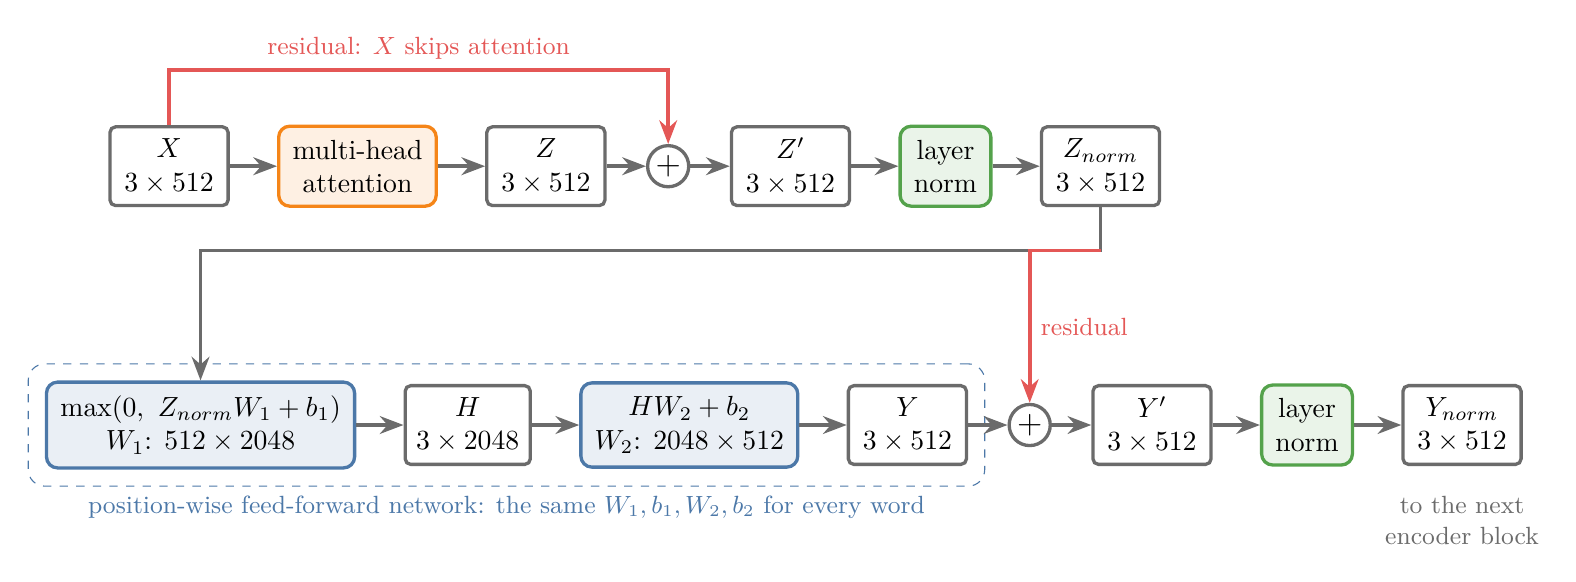
\begin{tikzpicture}[every node/.append style={font=\sffamily},
  mat/.style={draw=cgrey, fill=white, rounded corners=2pt, align=center, inner sep=4pt, minimum width=1.5cm, minimum height=1.0cm},
  op/.style={box=#1, inner sep=5pt, minimum height=0.9cm},
  plus/.style={draw=cgrey, circle, inner sep=1pt, font=\large}]
  % row 1: attention half
  \node[mat] (X) at (0,0) {$X$\\$3 \times 512$};
  \node[op=corange, right=0.6cm of X] (mha) {multi-head\\attention};
  \node[mat, right=0.6cm of mha] (Z) {$Z$\\$3 \times 512$};
  \node[plus, right=0.5cm of Z] (p1) {$+$};
  \node[mat, right=0.5cm of p1] (Zp) {$Z'$\\$3 \times 512$};
  \node[op=cgreen, right=0.6cm of Zp] (ln1) {layer\\norm};
  \node[mat, right=0.6cm of ln1] (Zn) {$Z_{\text{norm}}$\\$3 \times 512$};
  \draw[arrow] (X) -- (mha); \draw[arrow] (mha) -- (Z); \draw[arrow] (Z) -- (p1); \draw[arrow] (p1) -- (Zp);
  \draw[arrow] (Zp) -- (ln1); \draw[arrow] (ln1) -- (Zn);
  \draw[arrow, draw=cred] (X.north) -- ++(0,0.7) -| node[pos=0.25, above, text=cred, font=\sffamily\small] {residual: $X$ skips attention} (p1.north);
  % row 2: feed-forward half
  \node[op=cblue, below=2.2cm of X, xshift=0.4cm] (f1) {$\max(0,\ Z_{\text{norm}}W_1 + b_1)$\\$W_1$: $512 \times 2048$};
  \node[mat, right=0.6cm of f1] (Hm) {$H$\\$3 \times 2048$};
  \node[op=cblue, right=0.6cm of Hm] (f2) {$HW_2 + b_2$\\$W_2$: $2048 \times 512$};
  \node[mat, right=0.6cm of f2] (Y) {$Y$\\$3 \times 512$};
  \node[plus, right=0.5cm of Y] (p2) {$+$};
  \node[mat, right=0.5cm of p2] (Yp) {$Y'$\\$3 \times 512$};
  \node[op=cgreen, right=0.6cm of Yp] (ln2) {layer\\norm};
  \node[mat, right=0.6cm of ln2] (Yn) {$Y_{\text{norm}}$\\$3 \times 512$};
  \draw[arrow] (Zn.south) -- ++(0,-0.55) -| (f1.north);
  \draw[arrow] (f1) -- (Hm); \draw[arrow] (Hm) -- (f2); \draw[arrow] (f2) -- (Y); \draw[arrow] (Y) -- (p2); \draw[arrow] (p2) -- (Yp);
  \draw[arrow] (Yp) -- (ln2); \draw[arrow] (ln2) -- (Yn);
  \draw[arrow, draw=cred] (Zn.south) ++(0,-0.55) -| node[pos=0.75, right, text=cred, font=\sffamily\small] {residual} (p2.north);
  \node[note, below=0.25cm of Yn] {to the next\\encoder block};
  \begin{scope}[on background layer]
    \node[draw=cblue, dashed, rounded corners=6pt, fit=(f1)(Hm)(f2)(Y), inner sep=6pt, label={[cblue, font=\sffamily\small]below:position-wise feed-forward network: the same $W_1, b_1, W_2, b_2$ for every word}] {};
  \end{scope}
\end{tikzpicture}
\end{document}
